\documentclass{standalone}
\usepackage{tikz}

\begin{document}
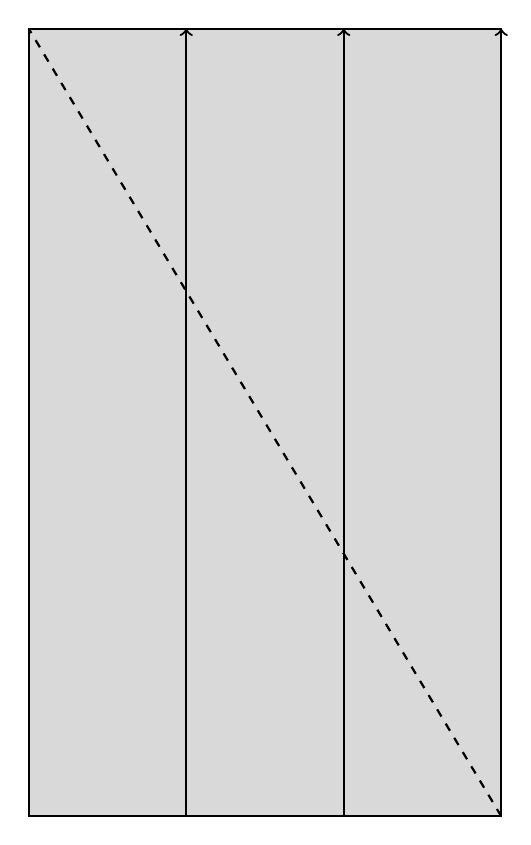
\begin{tikzpicture}[scale=2]
    % Dimensions of the rectangles
    \def\k{3} % width of the smaller rectangle
    \def\nk{5} % height of the smaller rectangle
    
    % Coordinates
    \coordinate (upper_left) at (0,0);
    \coordinate (upper_right) at (\k,0);
    \coordinate (lower_left) at (0,\nk);
    \coordinate (lower_right) at (\k,\nk);
    
    % Draw the larger rectangle R
    \draw[thick] (upper_left) rectangle (lower_right);
    
    % Draw the smaller rectangle r
    \draw[thick, fill=gray!30] (upper_left) rectangle (upper_right |- lower_left);
    
    % Draw the path from upper right to lower left
    \draw[dashed, thick] (upper_right) -- (lower_left);
    
    % Highlight the vertical steps
    \foreach \x in {1,...,\k} {
        \draw[thick, ->] (\x,0) -- (\x,\nk);
    }
\end{tikzpicture}
\end{document}